\documentclass[conference]{IEEEtran}
%\IEEEoverridecommandlockouts
% The preceding line is only needed to identify funding in the first footnote. If that is unneeded, please comment it out.
\usepackage{cite}
\usepackage{amsmath,amssymb,amsfonts}
\usepackage{algorithmic}
\usepackage{graphicx}
\usepackage{float}
\usepackage{textcomp}
\usepackage{xcolor}
\usepackage[british]{babel}
\def\BibTeX{{\rm B\kern-.05em{\sc i\kern-.025em b}\kern-.08em
		T\kern-.1667em\lower.7ex\hbox{E}\kern-.125emX}}
\begin{document}

\title{FPGA Based Prototyping of an ADPLL Network.\\}

\author{\IEEEauthorblockN{C. Dooley, E. Blokhina, B. Mulkeen}
	\IEEEauthorblockA{\textit{School of Electronic Engineering} \\
		\textit{University College Dublin}\\
		Belfield, Dublin 4, Ireland. \\
		email address} %TODO
}

\maketitle

\begin{abstract}
	This document is a model and instructions for \LaTeX.
	This and the IEEEtran.cls file define the components of your paper [title, text, heads, etc.]. *CRITICAL: Do Not Use Symbols, Special Characters, Footnotes, 
	or Math in Paper Title or Abstract.
\end{abstract}

\begin{IEEEkeywords}
	FPGA, ADPLL, Simulation, Prototype
\end{IEEEkeywords}
\section{Motivation}
The technical motivation underlying this paper is the creation of an Field Programmable Gate Array (FPGA) based prototyping platform for All Digital Phase Lock Loop (ADPLL) networks. As the creation of Application Specific Integrated Circuits (ASICs) is an expensive and time consuming process, any mistake has the potential to be rather costly. As such prior to the manufacture of an IC it is important to ensure that any errors made in the design have been weeded out prior to this stage.
Simulations at either at theoretical or gate/transistor levels have global usage in minimising such errors due to the ubiquity of simulators and their ease of use.\\
However simulations are only as good as the model used to describe the dynamics of the system, and emulating real jitter and other behaviours of a complex system is a rather difficult task. %TODO wording of this last sentence
An FPGA based prototype allows the system designers to validate the performance of both design and simulation, particularly the response to key noise sources such as power supply noise. An FPGA is ideal for this task as it leverages the existing skill set of a digital designer, permits the re-use of certain blocks, and most importantly enables cost effective and rapid reworking of the design.\\
An FPGA as a prototyping tool has seen use in the work of Dimitri Galayko and his research group in UPMC Sorbonne and in Elena Blokhina's team in University College Dublin, and has been used in the testing of established designs prior to their implementation in custom silicon\cite{zianbetov2013phd,shan2014phd}, the creation of realistic models for use in high level simulations\cite{theboys2019} and the exploration of new designs for digital blocks before progressing on to true digital design on a gate level.  %TODO references
In the case of Shan et. al \cite{shan2014phd} direct testing of control parameters was performed using an FPGA based design where all parameters were scaled down proportionally and thus the ideal gains for the loop filter found in simulation could be tested in a more realistic setting.\\
Similarly Koskin et. al \cite{theboys2019} used the analysis of a number of ADPLLs implemented on an FPGA both independently and in a network to validate previously obtained theoretical results while avoiding the costs associated with the development of a custom IC.\\
Prototyping on an FPGA does have its drawbacks, most notably the mixed-signal circuits central to the operation of an ADPLL are not implementable on an FPGA and while most fundamental digital circuit elements are present these elements are not true transistor level implementations of their functionality but rather implemented by lookup tables and other multi-role structures on the FPGA. These drawbacks present a challenge to a designer as they restrict the potential architectures of key blocks. This is of particular concern when trying to mimic the behaviour of an established design on an FPGA.\\
The particular system that this paper will discuss is an ADPLL network. Based on an idea first proposed in a 1995 paper by Pratt and Nguyen \cite{pratt1995distributed}, in which they proposed an alternative clock distribution network for ICs using a Cartesian grid of clocking areas, each with their own Phase Lock Loop, which has become known as a PLL Network . This methodology was implemented by Gutnik et. al \cite{gutnik2000active} who found it to be feasible. Subsequently Javiden et. al
\cite{javidan2011all} proposed the implementation of such a system using All Digital PLLs which better suited the use cases of the technology and avoided some of the flaws pointed out in the original paper.\\
This paper will examine the process of creating such a system, highlight the differences between potential designs and address some of the challenges and pitfalls that may be encountered along the way. This paper will also demonstrate that FPGA based prototyping can play a central role on the pathway to the implementation of an ADPLL network on a custom chip, or indeed any number of similar applications. The paper is organised as follows: Section II describes the system that will be used on the FPGA and Section III the implementation thereof and the challenges encountered in the process. Finally Section IV will present example measurements made on the platform and discuss their merit.

\section{System Architecture}
An ADPLL network as the name would suggest is created from a number of ADPLLs that coupled using digital phase comparators which attempt to measure the phase error between two oscillators, with each non edge node being connected to four neighbours. Figure \ref{fig:adpll_network} illustrates such a system on a small scale, with a number of ADPLLs laid out in a Cartesian grid. The individual ADPLLs, often called distributed ADPLLs as the phase detectors are shared between nodes, are made up of a digitally controllable oscillator, an error combination block and a digital loop filter with the aforementioned digital phase detectors lying between each pair of oscillators.
\begin{figure}[h]
	\centering
	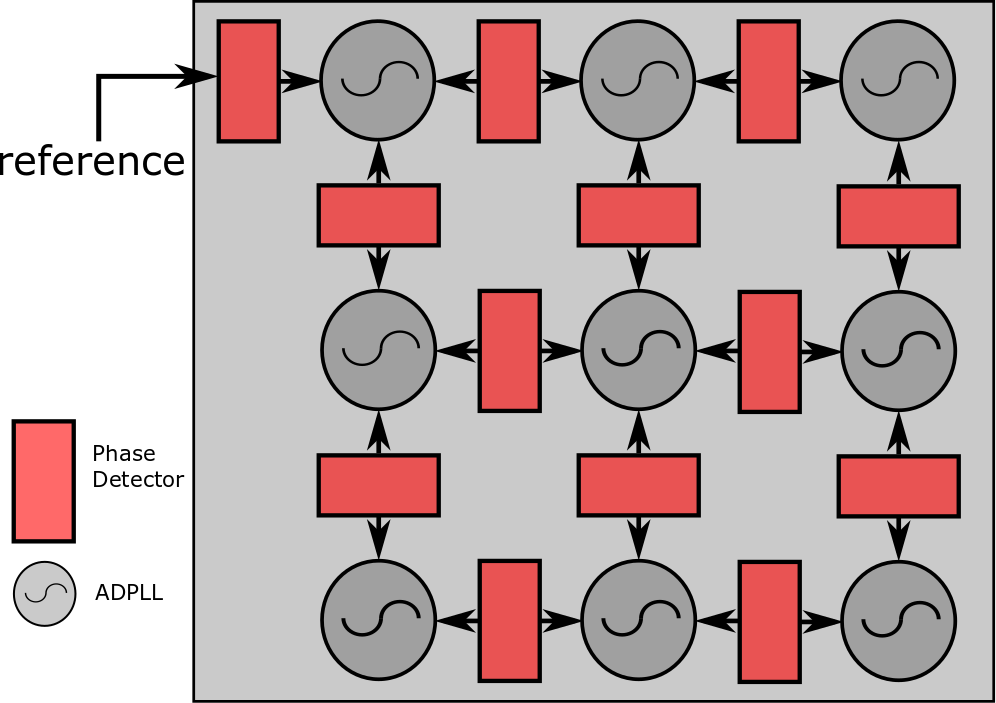
\includegraphics[width=0.25\textwidth]{adpll_network}
	\caption{ADPLL Network Architecture.}
	\label{fig:adpll_network}
	\vspace{0.5cm}
	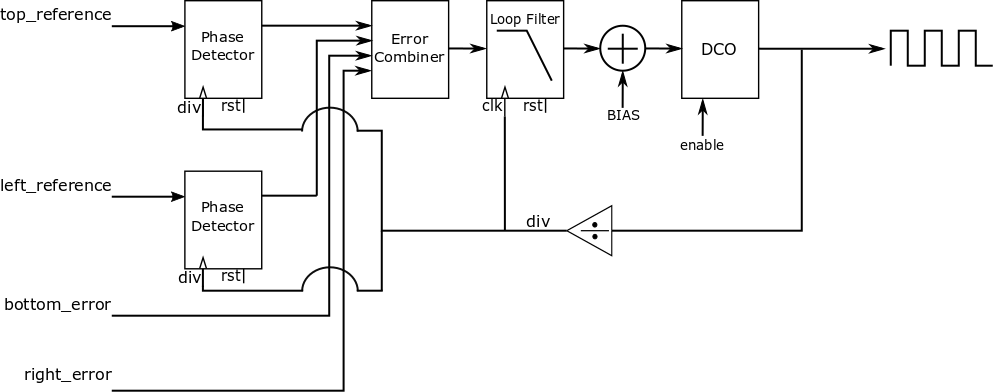
\includegraphics[width=0.4\textwidth]{dist_adpll}
	\caption{Distributed ADPLL Design.}
	\label{fig:adpll_base}
\end{figure}
\subsection{Digitally Controlled Oscillators}
While regular Voltage Controlled Oscillator (VCO) is tuned by the input voltage over a continuous range of values in a digital system there are a very limited number of voltages representable, most commonly just two levels. As such using the voltage itself to control an oscillator is not a viable strategy and instead Digitally, or as they are sometimes known as Numerically, Controlled Oscillators (DCO) accept an \textit{n} bit wide control signal that alters the period of the output waveform. While tuning range, centre frequency and linearity apply as in a VCO, a DCO also has a minimum frequency step as a result of the non continuous control values. %TODO WORDING
In combination with the bit width of the control signal the minimum frequency step limits the range over which the oscillator can be tuned. Frequently the output of the DCO is divided down to allow the control blocks in the feedback path that are clocked on this signal to run at a lower and thus easier frequency.
\subsection{Loop Filter}
The loop filter is a key aspect of a phase lock loop as without it only the current output of the phase detector could be used to compute the control voltage of the VCO.
In an ADPLL it performs an identical role, however the digital environment results the traditional loop filter being replaced by a discrete time Proportional Integral (PI) controller, with the integral path of the controller implemented by an accumulator.
\subsection{Error Combiner}
The Error Combiner, as the name suggests, performs a summation of the error signals from the phase detectors lying between any neighbouring oscillator and its neighbours. It is often convenient for this to be performed as a weighted sum, thus avoiding different gain requirements for the loop filter of oscillators in the corners of the grid that only have a pair of neighbours. The ability to change the weights during operation enables ``uni-directional start-up'' which Javiden et. al
\cite{javidan2011all} found prevented the system from entering unwanted stable equilibriums warned of in Pratt' and Nguyen's seminal paper.
\subsection{Phase Detector}
As in a conventional PLL the phase detector outputs a value proportional to the difference in phase between a pair of signals, which is then output as a continuous voltage.
A digital phase detector then attempts to do the same by measuring the difference between fixed reference points in the waveform, which as a digital system deals with square waves this is typically the rising edge of each input to the block.
Similarly to the oscillator quantisation also plays a role in the behaviour of this block, with the time difference between each rising edge having a minimum possible measurement step.
In distributed ADPLLs the phase detector has dual outputs, each the inverse of the other, in order to feed the correct value to both of the connected error combiners. 

\section{FPGA Prototyping}
\subsection{FPGA Restrictions}
The use of an FPGA comes with many restrictions as to how a complex system such as an ADPLL can be designed with the mixed signal blocks, the DCO and phase detectors, in particular being curtailed by the lack of transistor level control of the design and layout.\\
Two potential solutions exist which alleviate this problem, and are suited to different frequency ranges and/or goals of the designer. Firstly the clock signal generated by the FPGA's clock distribution block can be used to drive accumulator based oscillators and phase detectors a technique suitable in two main use cases: The emulation of the performance of an already designed system operating at a proportionally cut down frequency. At frequencies that are orders of magnitude lower than the maximum obtainable clock frequency of the FPGA's clock manager.
The downside of this approach is that the minimum steps are dictated by the clock frequency of the FPGA, which at frequencies that are not orders of magnitude lower than the FPGA clock will result in coarse resolutions for detector or oscillator, and thus greater jitter seen at the oscillator output.\\
The second solution to the problem is more akin to the real world system, and uses the delay through primitive elements such as inverters, which can be deduced from measurements on the FPGA of choice but will vary depending on the layout selected. In the case of the FPGA used for this paper, a Xilinx Artix-7 (XC7A100T-1CSG324C) this delay is in the region of 300 picoseconds but varies depending on the routing between elements. This design is better suited to scenarios where the desired operating frequency is a significant fraction of the maximum usable clock of the FPGA or it is particularly desirable to have asynchronous behaviour in the system as in an ASIC. It is not suited to lower frequency designs as the number of inverters required will run into spacial constraints.
\subsection*{Digitally Controlled Oscillators on an FPGA}

\newpage
\bibliography{conf.bib} 
\bibliographystyle{IEEEtran}

\end{document}


